% Final presentation slides — 5 min / 7 frames
% Geometrically Inductive SSL for EEG
% =============================================================================

\documentclass[aspectratio=169]{beamer}

\usepackage[utf8]{inputenc}
\usepackage{amsmath, amssymb}
\usepackage{booktabs}
\usepackage{tikz}
\usepackage{pgfplots}
\pgfplotsset{compat=1.18}
\usepackage{xcolor}

\usetikzlibrary{positioning, arrows.meta, calc}

\usetheme{metropolis}
% Fallback for environments without metropolis: comment the line above and
% uncomment the two below.
% \usetheme{default}
% \usecolortheme{whale}

% Common colors
\definecolor{geocolor}{HTML}{2E86AB}
\definecolor{codexcolor}{HTML}{A23B72}
\definecolor{chindcolor}{HTML}{888888}
\definecolor{winnercolor}{HTML}{18A558}
\definecolor{accentred}{HTML}{D7263D}

% Title meta
\title{Geometrically Inductive Self-Supervised Learning for EEG}
\subtitle{A Design Study of Spatial Attention Across Sessions, Subjects, and Montages}
\author{Tianxin Zhou}
\institute{ECEN 525 -- Brain--Computer Interaction \\ Santa Clara University}
\date{Spring 2026}

\begin{document}

% =============================================================================
% Slide 1 — Title
% =============================================================================
\begin{frame}[plain]
  \titlepage
  \vfill
  \centering
  \footnotesize
  \texttt{github.com/tianxin-scu/geometric-eeg-ssl}
\end{frame}

% =============================================================================
% Slide 2 — Problem statement
% =============================================================================
\begin{frame}{Problem: EEG is non-stationary -- by default}
  \vspace{-0.4em}
  \begin{columns}[T]
    \begin{column}{0.42\textwidth}
      \small
      EEG drifts on \textbf{three geometric axes}:
      \begin{itemize}
        \setlength{\itemsep}{2pt}
        \item \textbf{Session} — cap shifts day to day.
        \item \textbf{Subject} — head sizes differ; \texttt{C3} is not the same point.
        \item \textbf{Montage} — 2 to 256 electrodes in different layouts.
      \end{itemize}
      \vspace{0.4em}
      \footnotesize
      \textcolor{codexcolor}{\textbf{Codex models}} (LaBraM, EEGPT):
      identity-indexed embeddings.
      \textcolor{chindcolor}{\textbf{Channel-independent}} (BIOT):
      no spatial structure at all.
      \\[0.3em]
      Neither uses scalp geometry as an \emph{input}.
    \end{column}
    \begin{column}{0.56\textwidth}
      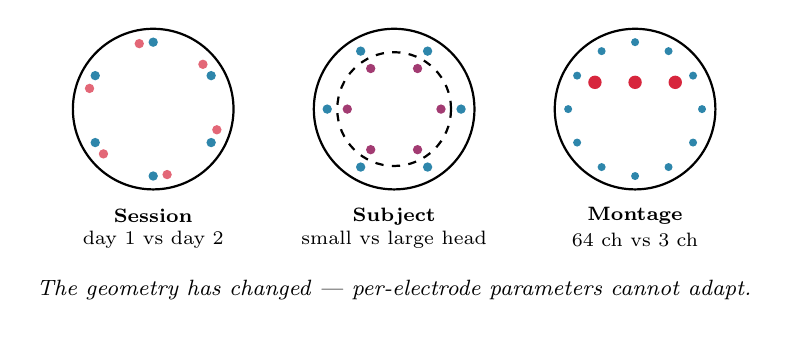
\begin{tikzpicture}[scale=0.85, every node/.style={font=\scriptsize}]
        % Three heads side by side showing the three drift axes
        \foreach \x/\lbl/\sub in {0/Session/{day 1 vs day 2}, 3.6/Subject/{small vs large head}, 7.2/Montage/{64 ch vs 3 ch}} {
          \draw[thick] (\x,0) circle (1.2);
          \node at (\x,-1.6) {\textbf{\lbl}};
          \node at (\x,-1.95) {\sub};
        }
        % Session: shifted electrodes
        \foreach \a in {30, 90, 150, 210, 270, 330} {
          \fill[geocolor]   ({0  + 1.0*cos(\a)}, {0 + 1.0*sin(\a)}) circle (0.07);
          \fill[accentred!70] ({0  + 1.0*cos(\a+12)}, {0 + 1.0*sin(\a+12)}) circle (0.07);
        }
        % Subject: small head outline vs large; same labels, different scale
        \draw[thick, dashed] (3.6,0) circle (0.85);
        \foreach \a in {0, 60, 120, 180, 240, 300} {
          \fill[geocolor] ({3.6 + 1.0*cos(\a)}, {0 + 1.0*sin(\a)}) circle (0.07);
          \fill[codexcolor] ({3.6 + 0.7*cos(\a)}, {0 + 0.7*sin(\a)}) circle (0.07);
        }
        % Montage: dense vs sparse
        \foreach \a in {0, 30, 60, ..., 330} {
          \fill[geocolor] ({7.2 + 1.0*cos(\a)}, {0 + 1.0*sin(\a)}) circle (0.06);
        }
        \fill[accentred] (6.6, 0.4) circle (0.10);
        \fill[accentred] (7.2, 0.4) circle (0.10);
        \fill[accentred] (7.8, 0.4) circle (0.10);
        % Caption
        \node[align=center, font=\footnotesize\itshape] at (3.6,-2.7) {The geometry has changed --- per-electrode parameters cannot adapt.};
      \end{tikzpicture}
    \end{column}
  \end{columns}
\end{frame}

% =============================================================================
% Slide 3 — Solution: geometry-conditioned attention
% =============================================================================
\begin{frame}{Solution: spatial attention conditioned on $g_{ij}$}
  \vspace{-0.3em}
  \begin{columns}[T]
    \begin{column}{0.42\textwidth}
      \small
      \textbf{Geometric descriptor.}
      \[
        g_{ij} = \big[\,\|p_i - p_j\|,\; p_i - p_j\,\big] \in \mathbb{R}^4
      \]
      Distance + signed displacement. No per-electrode parameters; same function for any montage.
      \\[0.4em]
      \textbf{Three options for where $g_{ij}$ enters:}
      \begin{itemize}
        \setlength{\itemsep}{2pt}
        \item \textbf{G1} (score) -- ``which electrodes attend''
        \item \textbf{G2} (value) -- ``what they exchange''
        \item \textbf{G3} (both)  -- combined
      \end{itemize}
      \footnotesize
      Training: BYOL-style momentum alignment + masked-patch reconstruction (EEGPT recipe).
    \end{column}
    \begin{column}{0.56\textwidth}
      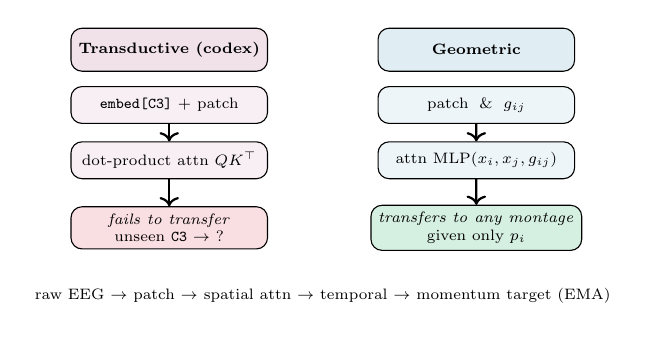
\begin{tikzpicture}[scale=0.78, every node/.style={font=\scriptsize}, transform shape]
        % Left -- transductive
        \node[draw, fill=codexcolor!15, rounded corners, minimum width=3.2cm, minimum height=0.7cm] (cT) at (0,3.5) {\textbf{Transductive (codex)}};
        \node[draw, fill=codexcolor!8, rounded corners, minimum width=3.2cm, minimum height=0.6cm] (cI) at (0,2.6) {\texttt{embed[C3]} $+$ patch};
        \node[draw, fill=codexcolor!8, rounded corners, minimum width=3.2cm, minimum height=0.6cm] (cQK) at (0,1.7) {dot-product attn $QK^\top$};
        \node[draw, fill=accentred!15, rounded corners, minimum width=3.2cm, minimum height=0.6cm, align=center] (cFail) at (0,0.6) {\scriptsize \emph{fails to transfer}\\ \scriptsize unseen \texttt{C3} $\to$ ?};
        \draw[->, thick] (cI) -- (cQK);
        \draw[->, thick] (cQK) -- (cFail);

        % Right -- geometric
        \node[draw, fill=geocolor!15, rounded corners, minimum width=3.2cm, minimum height=0.7cm] (gT) at (5,3.5) {\textbf{Geometric}};
        \node[draw, fill=geocolor!8, rounded corners, minimum width=3.2cm, minimum height=0.6cm] (gI) at (5,2.6) {patch $\;\&\;$ $g_{ij}$};
        \node[draw, fill=geocolor!8, rounded corners, minimum width=3.2cm, minimum height=0.6cm] (gA) at (5,1.7) {attn MLP$(x_i, x_j, g_{ij})$};
        \node[draw, fill=winnercolor!18, rounded corners, minimum width=3.2cm, minimum height=0.6cm, align=center] (gOK) at (5,0.6) {\scriptsize \emph{transfers to any montage}\\ \scriptsize given only $p_i$};
        \draw[->, thick] (gI) -- (gA);
        \draw[->, thick] (gA) -- (gOK);

        % Training pipeline ribbon
        \node[font=\scriptsize] at (2.5,-0.5) {raw EEG $\to$ patch $\to$ spatial attn $\to$ temporal $\to$ momentum target (EMA)};
      \end{tikzpicture}
    \end{column}
  \end{columns}
\end{frame}

% =============================================================================
% Slide 4 — In-distribution results + ablation
% =============================================================================
\begin{frame}{In-distribution: geometric $=$ codex $>$ channel-independent. G3 wins.}
  \begin{columns}[T]
    \begin{column}{0.5\textwidth}
      \centering
      \textbf{E1 -- PhysioNet MI LOSO (n=105)}\\[0.2em]
      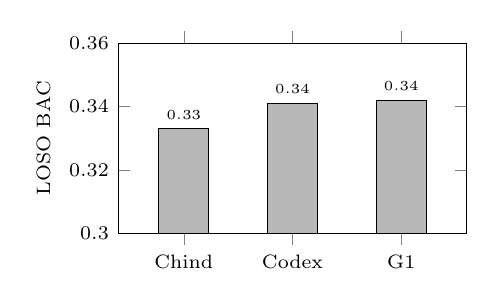
\begin{tikzpicture}
        \begin{axis}[
          width=6.0cm, height=4.0cm,
          ybar, bar width=18pt,
          ylabel={LOSO BAC}, ylabel near ticks,
          ymin=0.30, ymax=0.36,
          symbolic x coords={Chind, Codex, G1},
          xtick=data,
          enlarge x limits=0.3,
          nodes near coords,
          nodes near coords style={font=\tiny},
          tick label style={font=\scriptsize},
          label style={font=\scriptsize},
        ]
          \addplot[fill=chindcolor!60] coordinates {(Chind,0.333) (Codex,0.341) (G1,0.342)};
          \draw[dashed, gray] (axis cs:Chind,0.25) -- (axis cs:G1,0.25);
        \end{axis}
      \end{tikzpicture}\\[0.1em]
      \scriptsize Wilcoxon (G1 vs codex): $p = 0.911$
    \end{column}
    \begin{column}{0.5\textwidth}
      \centering
      \textbf{E5 -- G1 / G2 / G3 ablation}\\[0.2em]
      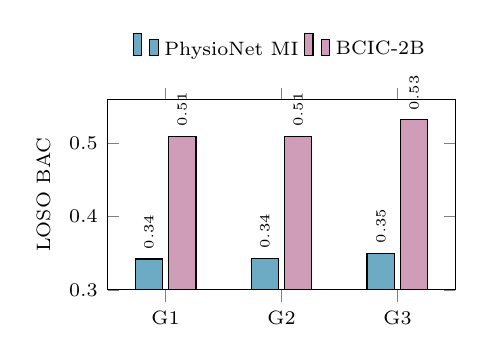
\begin{tikzpicture}
        \begin{axis}[
          width=6.0cm, height=4.0cm,
          ybar=2pt, bar width=10pt,
          ylabel={LOSO BAC}, ylabel near ticks,
          ymin=0.30, ymax=0.56,
          symbolic x coords={G1, G2, G3},
          xtick=data,
          enlarge x limits=0.25,
          legend style={font=\scriptsize, at={(0.5,1.15)}, anchor=south, legend columns=2, draw=none},
          tick label style={font=\scriptsize},
          label style={font=\scriptsize},
          nodes near coords,
          nodes near coords style={font=\tiny, rotate=90, anchor=west},
        ]
          \addplot[fill=geocolor!70] coordinates {(G1,0.342) (G2,0.343) (G3,0.350)};
          \addplot[fill=codexcolor!50] coordinates {(G1,0.509) (G2,0.509) (G3,0.532)};
          \legend{PhysioNet MI, BCIC-2B}
        \end{axis}
      \end{tikzpicture}\\[0.1em]
      \scriptsize \textbf{G3} (geometry at \emph{both} score and value) wins on both datasets.
    \end{column}
  \end{columns}
  \vspace{0.4em}
  \footnotesize
  \begin{itemize}
    \setlength{\itemsep}{1pt}
    \item In-distribution: geometric and codex tie; both beat channel-independent.
    \item Within geometric: G3 dominates G1/G2 -- geometry contributes a small signal at each slot it enters.
  \end{itemize}
\end{frame}

% =============================================================================
% Slide 5 — Cross-montage results (headline)
% =============================================================================
\begin{frame}{Cross-montage transfer (64\,ch $\to$ 3\,ch): codex-nn matches geometric}
  \vspace{-0.2em}
  \begin{columns}[T]
    \begin{column}{0.56\textwidth}
      \centering
      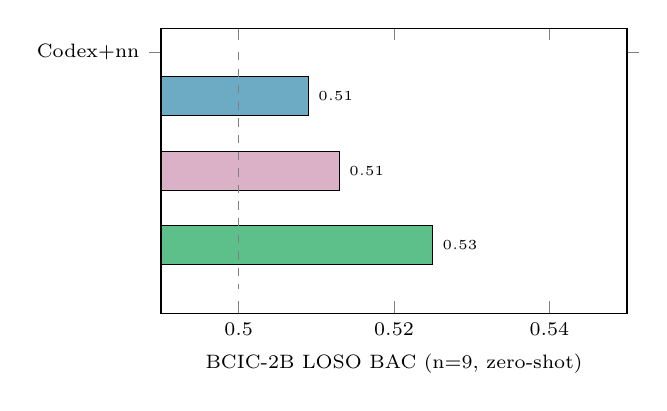
\begin{tikzpicture}
        \begin{axis}[
          width=7.5cm, height=5.2cm,
          xbar, bar width=14pt,
          xlabel={BCIC-2B LOSO BAC (n=9, zero-shot)},
          xmin=0.49, xmax=0.55,
          symbolic y coords={CodexNN, CodexRand, GeoG1},
          ytick=data,
          yticklabels={Codex+nn, Codex+random, G1 geometric},
          nodes near coords,
          nodes near coords style={font=\tiny},
          tick label style={font=\scriptsize},
          label style={font=\scriptsize},
        ]
          \addplot[fill=geocolor!70]   coordinates {(0.509,GeoG1)};
          \addplot[fill=codexcolor!40] coordinates {(0.513,CodexRand)};
          \addplot[fill=winnercolor!70] coordinates {(0.525,CodexNN)};
          % Chance line at 0.50
          \draw[dashed, gray] (axis cs:0.50,GeoG1) -- (axis cs:0.50,CodexNN);
        \end{axis}
      \end{tikzpicture}\\[-0.1em]
      \scriptsize Chance = 0.50 (binary). Dashed line = chance.
    \end{column}
    \begin{column}{0.42\textwidth}
      \small
      \textbf{The proposal's headline test:}\\
      \emph{Pretrain on PhysioNet MI (64\,ch);
      zero-shot transfer to BCIC-2B (3\,ch).}
      \\[0.6em]
      \textcolor{winnercolor}{\textbf{Codex + nearest-neighbour fallback}} (0.525) slightly \textbf{beats} the geometric encoder (0.509).
      \\[0.4em]
      The nn fallback uses 3-D coordinates to assign each unseen electrode to its closest pretraining entry -- it exploits \emph{the same geometry} at transfer time, without learning a geometric attention bias.
      \\[0.4em]
      \footnotesize\textit{The predicted ordering inverts.}
    \end{column}
  \end{columns}
\end{frame}

% =============================================================================
% Slide 6 — Conclusion + future work
% =============================================================================
\begin{frame}{Conclusion: an honest read, a sharper target}
  \begin{columns}[T]
    \begin{column}{0.52\textwidth}
      \small
      \textbf{What we learned:}
      \begin{itemize}
        \setlength{\itemsep}{2pt}
        \item Spatial structure helps; geometric $=$ codex at pilot scale.
        \item \textbf{G3} is the strongest geometric configuration.
        \item \textbf{Codex + nn} is a tougher transfer baseline than the proposal anticipated.
      \end{itemize}
      \vspace{0.4em}
      \textbf{Three concrete next steps:}
      \begin{enumerate}
        \setlength{\itemsep}{2pt}
        \item Push G3 with \textbf{richer descriptors} (spherical, geodesic).
        \item \textbf{Scale up} pretraining and re-run E2c.
        \item Test on \textbf{high-density montages} where codex-nn breaks down.
      \end{enumerate}
    \end{column}
    \begin{column}{0.46\textwidth}
      \centering
      \footnotesize
      \textbf{Predicted vs.\ observed}\\[0.3em]
      \begin{tabular}{lcc}
        \toprule
                          & \textbf{Predicted} & \textbf{Observed} \\
        \midrule
        In-distribution   & tie            & \textcolor{winnercolor}{\textbf{tie}} \\
        Cross-subject     & geometric $+$  & tie \\
        Cross-montage     & geometric $++$ & codex-nn $\approx +$ \\
        \bottomrule
      \end{tabular}
      \\[1.0em]
      \scriptsize
      \texttt{github.com/tianxin-scu/}\\\texttt{geometric-eeg-ssl}
    \end{column}
  \end{columns}
\end{frame}

% =============================================================================
% Slide 7 — Key references
% =============================================================================
\begin{frame}{Key References}
  \footnotesize
  \begin{itemize}
    \setlength{\itemsep}{3pt}
    \item Wang et al. \textbf{EEGPT}. NeurIPS 2024 -- training recipe (momentum + reconstruction).
    \item Grill et al. \textbf{BYOL}. NeurIPS 2020 -- momentum-encoder alignment.
    \item He et al. \textbf{MAE}. CVPR 2022 -- masked-patch reconstruction.
    \item Hamilton, Ying, Leskovec. \textbf{GraphSAGE}. NeurIPS 2017 -- inductive vs. transductive vocabulary.
    \item Veli\v{c}kovi\'c et al. \textbf{GAT}. ICLR 2018 -- attention over relational features.
    \item Jiang et al. \textbf{LaBraM}. ICLR 2024; Yang et al. \textbf{BIOT}. NeurIPS 2023 -- codex / channel-independent baselines.
    \item Schalk et al. 2004 -- PhysioNet MI; Tangermann et al. 2012 -- BCIC-2B; Kemp et al. 2000 -- Sleep-EDF.
  \end{itemize}
  \vspace{0.6em}
  \centering
  \scriptsize
  Full reference list and per-experiment details in the project report.
\end{frame}

\end{document}
